\chapter{Big Data Defined}
The intended outcome of this literature review is to deliver a thorough explanation of the various technologies used throughout the project and to provide details on any additional subject matter aspects which will aid the understanding of the project. 

A general summation of Big Data and its application is given in section \ref{bigdata} which is followed by a discussion on the pre-processing of datasets discussed in section \ref{etl}. A high level overview of the NoSQL concept is examined in section \ref{nosql}. The various types of dataset classification which are utilised in the project are given in section \ref{dbclass}.

\section{Big Data}\label{bigdata}
Big Data is a broad, evolving term bound to a complex and powerful application of analytical insight which over recent years has had a variety of definitions. In simplistic terms Big Data can be described as extremely large datasets that may be studied computationally to reveal patterns, trends, and associations for ongoing discovery and analysis.

The 2011 McKinsey Global Institute (MGI), a multinational management consultancy firm, compiled a report namely ``Big data: The next frontier for innovation, competition, and productivity" outlines the potential effects big data will have on a number of industries. The report suggests that with the increasing ``exponential" growth of data volume, simply recruiting a ``few data-orientated managers" will be a temporary fix rather than a lasting solution. MGI suggest that if companies in a variety of sectors, such as the healthcare and retail industry, were to take advantage of the value which big data brings could see potentially huge returns. ``...a retailer using big data to the full could increase its operating margin by more than 60 percent" \cite{mckinskey}. The report also states that if ``healthcare were to use big data creatively and effectively to drive efficiency and quality, the sector could create more than \$300 billion in value every year" \cite{mckinskey}. Thus further cementing the view which accepts that big data plays a pivotal role in everyday modern life.

\subsection{5vs Model}
In 2001, Gartner analyst Doug Laney delivered the \textit{3vs model} which defines the challenges and opportunities which have arisen from the increase in data volume. Laney categorises big data into three dimensions; Volume, Velocity and Variety, with the increase of each encapsulating the challenges currently faced today of big data management. \begin{figure}[h]\begin{center}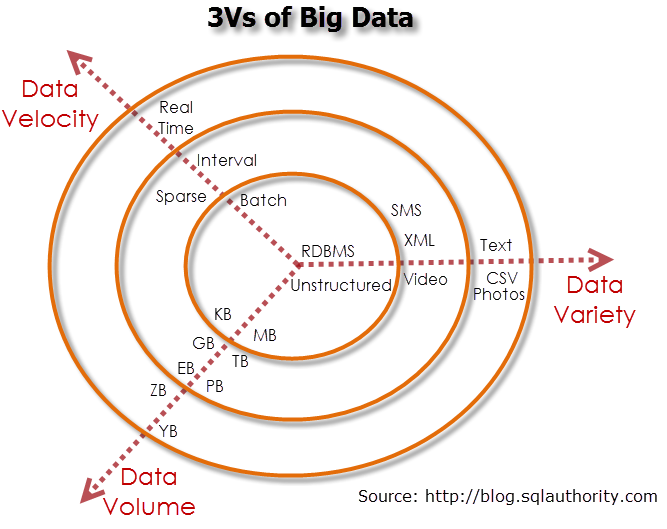
\includegraphics[width=0.8\linewidth]{images/3vs}\caption{3vs data model}\label{fig:3vs}\end{center}\end{figure}

\parindent 0pt The characteristics of each property illustrated in figure \ref{fig:3vs} are defined as: \textbf{Volume} - The vast amounts of data generated every second. With the creation and storage of large quantities of data, the scale of this data becomes progressively vast. \textbf{Velocity} -  The speed at which new data is generated and the speed at which data moves around emphasising the ``timeliness" of the big data. In order to fully profit from the commercial value of big data, data collection and data examination must be conducted promptly . \textbf{Variety} - This characteristic alludes to the various types of data we can now use; semi-structured and unstructured. Examples being ``audio, video, webpage and text as well as traditional structured data" \cite{bigdata}.

\parindent 15pt Big Data is a term becoming increasingly common in business and society. Overcoming obstacles and implementing effective, actionable Big Data strategies is key for successful big data management. In recent years a fourth category was introduced; \textbf{Veracity} - Data inconsistencies and incompleteness result in data uncertainty and unreliability; which creates a new challenge, keeping data organised \cite{bigdata}.

The final and considered by many to be the most important \textit{V} of big data is \textbf{Value}. ``All the volumes of fast-moving data of different variety and veracity have to be turned into value" \cite{ibm}. One of the biggest challenges faced by organisations is having the ability to turn data into something useful. It can be an easy trap to fall into for a business aiming to embark on big data initiatives without a clear understanding of costs and benefits \cite{bigdata}. Thus the importance of establishing clear and achievable business objectives.

\begin{figure}[h]\begin{center}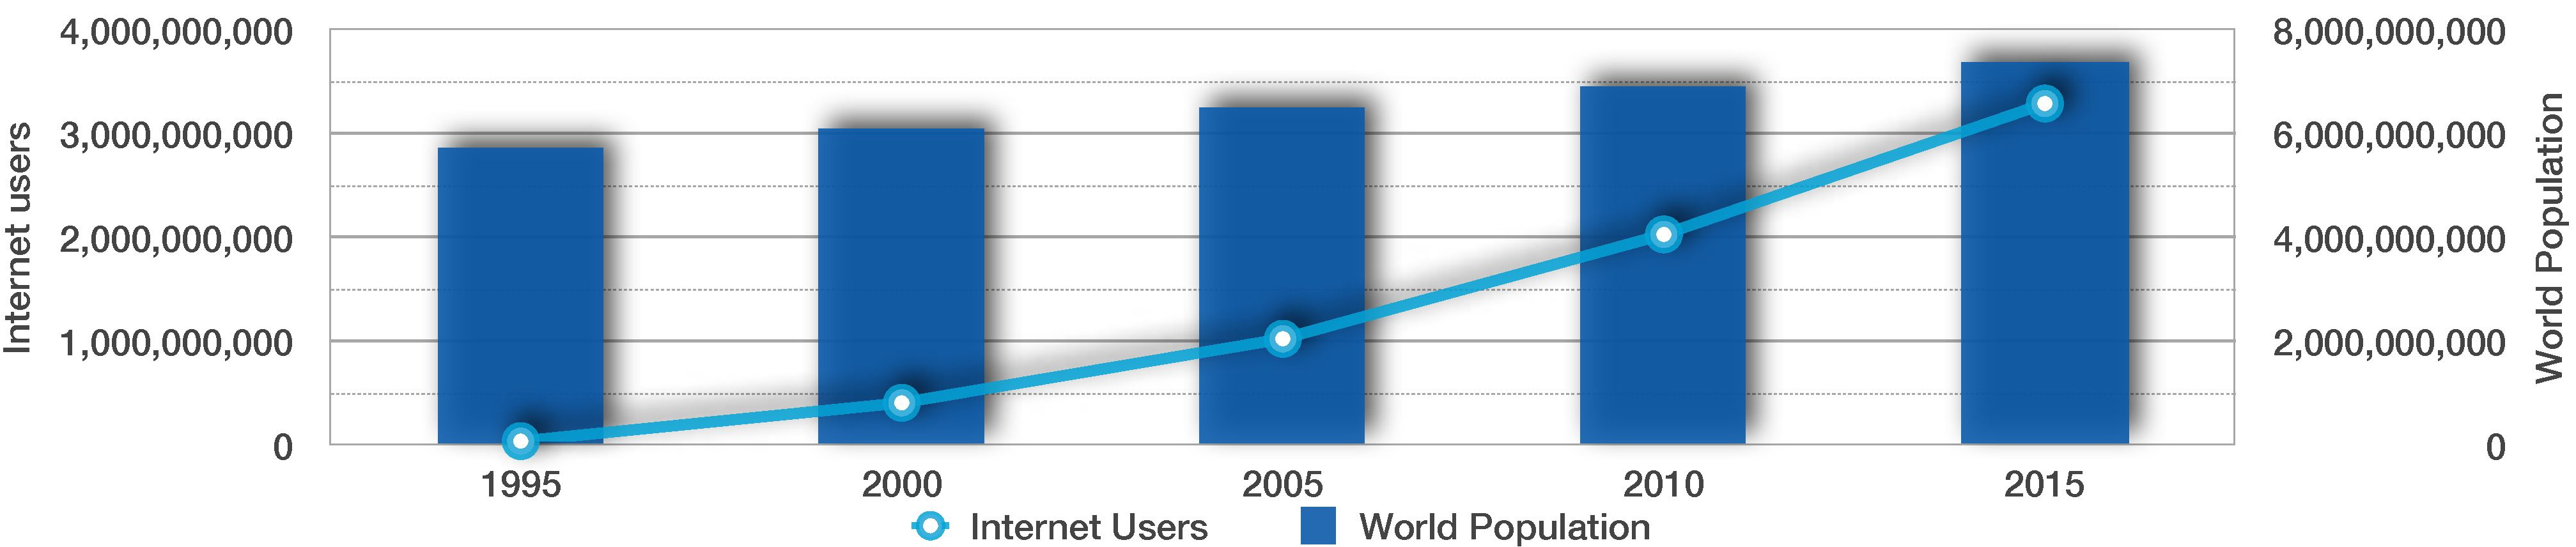
\includegraphics[height = 8cm,width=1\linewidth]{images/worldpopgraph}\caption{World population vs Internet users}\label{fig:worldpop}\end{center}\end{figure}
The amount of data produced has dramatically increased from when Laney first introduced the 3vs model in 2001. This is in no small part due to the availability and accessibility of the internet. In 1995 the internet had on average 45 million users, 1\% of the worlds population. This figure increased to over 1 billion people with internet access worldwide in 2005, and by 2010 nearly 2 billion which was 30\% of the worlds population. The latest figures show that in 2015 the penetration of the internet reached 3 billion people, 40\% of the entire population. Social media sites such as Facebook, Twitter, Snapchat, Instagram and Pinterest generate millions of  with Facebook boasting 1 million links shared, 2 million friend requests sent and 3 million messages sent on average every twenty minutes \cite{statref}. The graph and data table in figure \ref{fig:worldpop} illustrate the continual growth of internet accessibility as a whole. With this growth comes the challenge of an amalgamation of the benefit of high volumes of captured analytical data and using this data to add value to an organisation.






